\documentclass{school-22.101-notes}
\date{November 16, 2011}

\begin{document}
\maketitle


\topic{Decay Mechanism}
Three Basic Decay Types\footnote{See Krane 3.3, 6.1-6.5.} (see Figure~\ref{Z-N-grid}):
\begin{enumerate}
\item $\alpha$ decay:
Example: \ce{_{88}^{236} Ra \to ^{232}_{86} Rn + \alpha}, $T_{\alpha} = 4.8$ MeV, $t_{1/2} = 1600$ years. 
\item $\beta$ decay: beta plus decay is \ce{n \to p + e^- + \nu}, beta minus decay is \ce{p \to n + e^+ + \bar{\nu}}
\item $\gamma$ decay: \ce{X^* \to X + \gamma}, excited state to lower energy state.
\end{enumerate}
\begin{figure}[h]
    \centering
    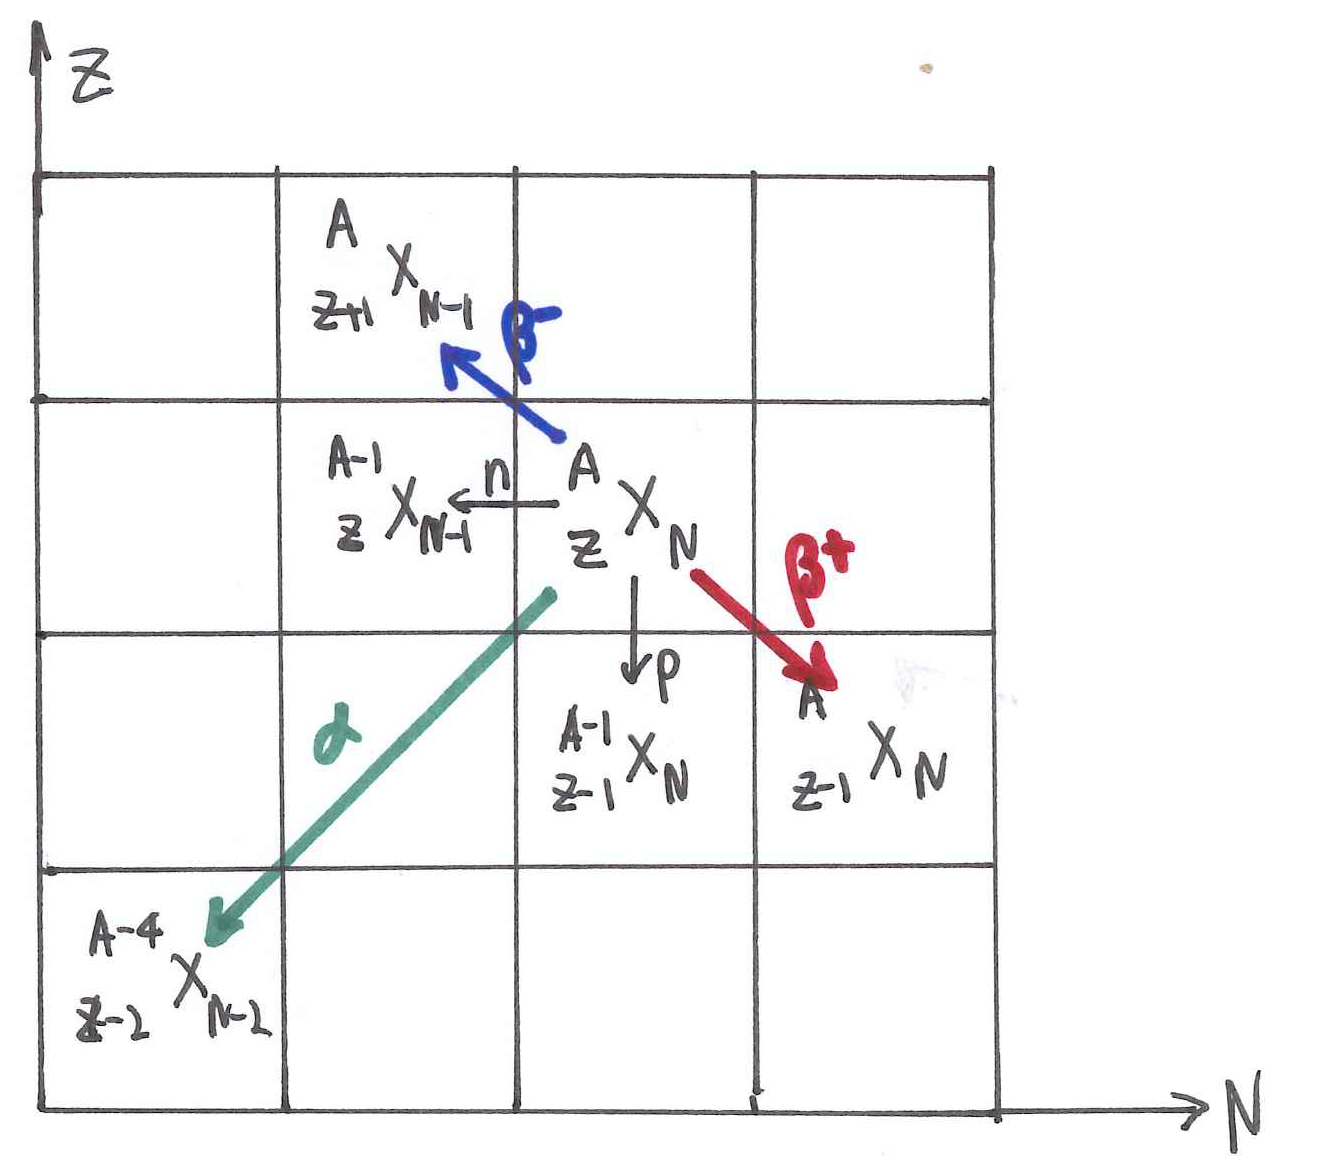
\includegraphics[width=3in]{images/rd/Z-N-grid.png}
    \caption{Radioactive Decay Demonstration \label{Z-N-grid}}
\end{figure}


Decay mechanisms: the decay constant describes probability of decay per unit time, and it is defined as, 
\eqn{ \lambda = -\frac{\dNdt}{N(t)} } 
\begin{align}
\dNdt (t) &= - \lambda N(t) &  N(t) &= N_0 e^{-\lambda  t} \\
N(t_{1/2}) &= \frac{1}{2} N(0) & t_{1/2} &= \frac{\ln 2}{\lambda} = \frac{0.693}{\lambda} \\
\mbox{mean lifetime }\tau &= \frac{\int_0^{\infty} t \left| \dNdt \right| \dt }{\int_0^{\infty}  \left| \dNdt \right| \dt} = \frac{1}{\lambda} & \tau &= \frac{1}{\lambda}
\end{align}

Various decay modes: 
\begin{enumerate}
\item Parent $N_1$ decay into daughter product$N_2$: 
\begin{align}
N_1 (t) &= N_0 e^{-\lambda t} \\
N_2 (t) &= N_0 - N_1 (t) = N_0 (1 - e^{-\lambda t}) 
\end{align}

\item Parent $N_1$ decay parallelly into daughters $N_{2,a}$ (with $\lambda_a$) and $N_{2,b}$ (with $\lambda_b$). The total decay constant is just $\lambda_t = \lambda_a + \lambda_b$. 
\begin{align}
N_1 (t) &= N_0 e^{-\lambda_t t} \\
N_{2,a} (t) &= \frac{\lambda_a}{\lambda_t} N_0 (1 - e^{-\lambda_t t}) \\
N_{2,b} (t) &= \frac{\lambda_b}{\lambda_t} N_0 (1 - e^{-\lambda_t t})
\end{align}

\item Parent $N_1$ decay into daughter $N_2$, which instantaneously decay into granddaughter $N_3$ through \ce{N_1 ->[\lambda_1] N_2 ->[\lambda_2] N_3}.
\begin{align}
\frac{\derivative N_1}{\dt} &= -\lambda_1 N_1 (t)   & N_1 (t) &= N_{0} e^{-\lambda_1 t} \\
\frac{\derivative N_2}{\dt} &= \lambda_1 N_1 (t) - \lambda_2 N_2(t)   & N_2 (t) &= N_{0} \frac{\lambda_1}{\lambda_2 - \lambda_1} \left( e^{-\lambda_1 t} - e^{-\lambda_2 t} \right) \\
\frac{\derivative N_3}{\dt} &= \lambda_2 N_2 (t)    & N_3 (t) &= N_{0} \frac{\lambda_1 \lambda_2}{\lambda_2 - \lambda_1} \left( \frac{1 - e^{-\lambda_1 t} }{\lambda_1} - \frac{1- e^{-\lambda_2 t}}{\lambda_2} \right) 
\end{align}
\end{enumerate}

%%%%%%%%%%%%%%%% Alpha Decay %%%%%%%%%%%%%%%%%%%%%%%%%
\topic{Alpha Decay} 
A few key points about alpha decay\footnote{See Krane 8, Liboff 4.2 and 4.5 for more details}:
\begin{enumerate} 
\item Why does the parent nuclei (typically heavy) want to spit out $\alpha$ particles? 

Answer: Coulomb Repulsion Effect. Coulomb force increases super-linearly with respect to binding energy\footnote{Nuclear binding energy $\propto a_V A,$ Coulomb repulsion $\propto -a_C \frac{Z^2}{A^{1/3}}$, Coulomb term increases faster than nuclear binding term for heavy nuclei.}. There is a need to get rid of some protons.  
\item $\alpha$-decay is the most favored form of radioactive decay among heavy nuclei. Very rare to observe other nucleon emission besides alpha particles. Why is the $\alpha$ particle chosen for spontaneously carrying away the positive charge?
    \begin{enumerate}
    \item \ce{^4_2 He_2} is doubly magic, very stable, tightly bound structure;
    \item \ce{^4_2 He_2} has relatively small mass compared with the mass of its separate constituents (beats \ce{^{12} C}, \ce{^{18} O}). It is favored as an emitted particle if we hope to have the disintegration products as light as possible and thus get the largest possible release of T. In addition, later we will find out $P_T = e^{-2G}$ decreases significantly as $m > m_{\alpha}, Z > Z_{\alpha}.$
    \end{enumerate}
\item To determine whether a decay mode is possible, we need to check three things:
    \begin{enumerate}
    \item Energetically allowed, that is, $Q > 0$. For instance, for U-232 (see Table~\ref{232-U}), \ce{^4 H} is the only energetically possible decay mode. Decay through emission of lighter particles is not possible because they require energy instead of release energy.
    \item $\lambda$ for the decay cannot be too small, $t_{1/2}$ cannot be too large (larger than $10^{16}$ years is no good). 
    \item Its $\beta$ decay $\lambda$ cannot be too much higher than $\alpha$ decay's, or it would mask the $\alpha$ decay. Most nuclei with $A>190$ (and many with $150 < A < 190$) are energetically possible for $\alpha$ decay, but only one-half can actually meet these requirements.
    \end{enumerate}
\item $\lambda$ and $t_{1/2}$ are very sensitive to Q. $\log t_{1/2} \propto \frac{1}{\sqrt{Q_{\alpha}}}$. Doubling Q may reduce the $t_{1/2}$ by a $10^{20}$ order of magnitude. Example, see Table~\ref{Th}. 
\item Why is decay via emission of heavier nuclei (such as \ce{^{16}O} or \ce{^{12}C}) rarely observed? 

Answer: $P_T = e^{-2G}, 2G \approx \sqrt{\frac{E_G}{Q}}, E_G \sim Z_1^2 Z_2^2$. Decaying via a heavier nuclei means $E_G$ is larger than that of $\alpha$ emission (because $Z_1, Z_2$ would be closer in value), making the probability decreases significantly. 
\item Why is decay via emission of lighter nuclei (such as \ce{^1H}, \ce{^2H}, \ce{^3He}) rarely observed?

Answer: $\alpha$ particle is favored over lighter nuclei because it is doubly magic stable, very stable, tightly bound. HW6 solution also says `this could be qualified by $Q_{\alpha}$ in $2G = \sqrt{\frac{E_G}{Q_{\alpha}}}$. 
\item Why is spontaneous fission not very likely?

Answer: spontaneous fission means $Z_1 \sim Z_2$, which makes the product large, $E_G$ large, $2G$ large, $P_T$ small. 
\end{enumerate}
%
\begin{table}
    \centering
    \begin{tabular}{|c|c|} \hline
    Emitted Particle& Energy Release Q (MeV) \\ \hline 
    \ce{^1 H} & -6.12 \\ \hline
    \ce{^2 H} & -10.70 \\ \hline
    \ce{^3 He} & -9.92 \\ \hline
    \ce{^4 He} & 5.41 \\ \hline
    \ce{^7 Li} & -1.94 \\ \hline
    \end{tabular}
    \caption{Energy Release from \ce{^{232} U} Emitting Different Particles \label{232-U}}
\end{table}
%
\begin{table}
\centering
\begin{tabular}{|c|c|c|} \hline
Particle & Q (MeV) & $t_{1/2}$ in s \\ \hline
\ce{^{218} Th} & 9.85 & $10^{-7}$ s  \\ \hline
\ce{^{232} Th} & 4 & $10^{17}$ s  \\ \hline 
\end{tabular}
\caption{Comparison of Q and half-lives of \ce{^{218} Th}, \ce{^{232} Th}\label{Th} }
\end{table}

\subtopic{Energies of alpha-decay}
Recall alpha decay process is \ce{^A_Z X_N \to ^4_2 He_2 + ^{A-4}_{Z-2} \Xp_{N-2}}. Apply Conservation of Energy:
\begin{align}
m_X c^2 &= m_{\Xp} c^2 + T_{\Xp} + m_{\alpha} c^2 + T_{\alpha} \\
(m_X - m_{\Xp} - m_{\alpha} ) c^2 &= B(\Xp) + B(\alpha) - B(X) =  T_{\Xp} + T_{\alpha} = Q \label{Q-alpha}
\end{align}
The decay will occur spontaneously only if $Q >0$. 

Apply Conservation of Linear Momentum:
\begin{align}
0 &= P_{\Xp} - P_{\alpha}  & P_{\Xp}^2 &= P_{\alpha}^2 \\
T_{\Xp} m_{\Xp} &= T_{\alpha} m_{\alpha}  & T_{\Xp} &= T_{\alpha} \frac{m_{\alpha}}{m_{\Xp}} \\
Q &= T_{\alpha} + T_{\alpha} \frac{m_{\alpha}}{m_{\Xp}}  & T_{\alpha} &= \frac{Q}{1 + \frac{m_{\alpha}}{m_{\Xp}}}  \approx \boxed{ Q \left( 1 - \frac{4}{A} \right) } \approx 98\% Q
\end{align}
Given $Q$, we can find $T_{\alpha}$. Keep in mind that around 98\% of the Q goes into T of the $\alpha$ particles, and only about 2\% goes into T of the daughter particle (because it is heavy), which comes out to be 100 keV typically. Having a large Q means the isotope is a strong $\alpha$ emitter. Typically we define a strong $\alpha$ emitter to have $A > 190$.

\subtopic{Theory of Alpha Emission: Gamow Theory, Pre-formed Alpha Particle}
Assumptions:
\begin{itemize}
\item The $\alpha$ particle is pre-formed: before emission it is held together with the daughter product; Assume the distance between the two is $a$. 
\item Within the volume of $r<a$ (short range), nuclear binding force dominates, which is attractive; 
\item Outside (long range), coulomb potential dominates which is repulsive. 
\end{itemize}
For $\alpha$ decay to happen, the energy available to the $\alpha$ particle has to be positive: $Q > 0$. There is a region from $r=a$ to $r=b$ that the maximum available T or Q is smaller than the Coulomb potential. Then quantum tunneling is our only bet. 
\begin{align}
\lambda_{\alpha}&=f \cdot P_T & \mbox{Decay Constant}&=\mbox{Frequency of bouncing off barrier} \times \mbox{Tunneling probability} \\
f &= \frac{v_{\alpha}}{a} = \frac{v_{\alpha}}{1.25 A^{1/3}} & v_{\alpha} &= \mbox{Relative velocity of $\alpha$ as it rattles inside the well}
\end{align}
If we plug in $V = -V_0 = -50 \MeV, Q_{\alpha} = 5 \MeV, T_{\alpha} = Q - V = 55 \MeV = \frac{1}{2} m_{\alpha} V_{\alpha}^2$, we can find that $f = 5 \times 10^{21} \s^{-1}$, which is a higher frequency than nuclear vibration frequency (around $10^{12} \sim 10^{14} \s^{-1}$). Now we can consider the tunneling probability $P_T$ from $r$ to $r +\dr$. 
\begin{align}
\derivative P_T &= \frac{|e^{-k_2 (r+\dr)}|^2}{|e^{-k_2 r}|^2} = e^{-2 k_2 \dr}, & k_2 &= \sqrt{\frac{2m(V (r) -Q)}{\hbar^2}} \\
P_T &= \prod_i \dP_{\tau} = \exp \left(-2 \int_a^b k_2 (r) \dr \right) = e^{-2 G}, & G&=\mbox{Gamow Factor} \\ 
G &= \int_a^b k_2 (r) \dr = \int_a^b \sqrt{\frac{2 \mu}{\hbar^2} \left( \frac{Z_{\alpha} Z_D e^2}{r} - Q_{\alpha} \right)} \dr, & x &= \frac{a}{b} \\
&= \sqrt{\frac{2 \mu}{\hbar^2 Q_{\alpha}}} (Z_{\alpha} Z_D e^2) \left[ \arccos \sqrt{x} - \sqrt{x(1-x)} \right]  &
&\xrightarrow{x < 1} \sqrt{\frac{2 \mu}{\hbar^2 Q_{\alpha}}} (Z_{\alpha} Z_D e^2) \left[ \frac{\pi}{2} - 2 \sqrt{x} \right] \\
2G &= \sqrt{ 
\underbrace{ \left(\frac{2 \pi e^2 Z_{\alpha} Z_D}{\hbar c}\right)^2 \frac{\mu c^2}{2} }_{\mbox{Gamow Energy } E_G} 
\frac{1}{Q}} \left[ 1 - \frac{4}{\pi} \sqrt{x} \right] &
&= \boxed{ \sqrt{\frac{E_G}{Q}} \left[ 1 - \frac{4}{\pi} \sqrt{x} \right] }
\end{align}

For \ce{^{238} U}, we calculate:
\begin{align}
\left[ 1 - \frac{4}{\pi} \sqrt{x} \right] &= 0.51 \\
E_G &= \left( \frac{2 \pi \times e^2 \times 2 \times 90}{197} \right)^2 \left( \frac{4 \times 234}{4 + 234} \times \frac{938}{2} \right) = 125,700 \MeV  \\
\sqrt{\frac{E_G}{Q}} &= \sqrt{ \frac{125700}{4.25} } = 172 \\
2 G &= 172 \times 0.51 = 88 \\
P_T &= e^{-88} = 6 \times 10^{-39} \\
\lambda_{\alpha} &= f \times P_T = 4 \times 10^{21} \s^{-1} \times 6 \times 10^{-39} = 2.4 \times 10^{-17} \s^{-1} \\
t_{1/2} &= \frac{0.693}{\lambda} = 3 \times 10^{16} \s = 10^9 \mbox{ yr} 
\end{align} 
Implications of Gamow's model:
\begin{enumerate}
\item Strong dependency on $Q$ because $E_G$ is so large (recall 125799 MeV for U238). Recall the graph we had that doubling $Q$ results in a $10^{20}$ change in $t_{1/2}$. 
\item The calculated $E_G$ is larger than the measured values (Table~\ref{Q-t}). Potential reason: we keep the nuclear radius $a$ fixed in $x = \frac{a}{b}$ term; though for A$>$230, nuclei have strongly deformed shapes, and calculated $t_{1/2}$ is very sensitive to $x$\footnote{in fact, typically we would measure $t_{1/2}$ to reverse engineer the nuclei radius.}. 
\begin{table}
    \centering
    \begin{tabular}{|c|c|c|} \hline
     & \ce{^{220} Th} & \ce{^{232} Th} \\ \hline
     Q (MeV) & 8.95 & 4.08 \\ \hline
     $t_{1/2}$, measured ($\s^{-1}$) & $10^{-5}$ & $10^{17}$ \\ \hline
     $t_{1/2}$, model ($\s^{-1}$) & $3 \times 10^{-7}$ & $10^{16}$ \\ \hline     
    \end{tabular}
    \caption{Half-lives Predicted from Gamow's Model vs. Measurements \label{Q-t}}
\end{table}
\item Why alpha-decay not \ce{^{12} C} decay? 
\begin{table}
    \centering
    \begin{tabular}{|c|c|c|c|} \hline
    & $(Z_{p} Z_D)^2$ & $\mu$-dependency & $P_T$ \\ \hline
    $\alpha$ &  $(2 (Z-2))^2 \sim 4Z^2$ & 3.9 & $\exp(-\sqrt{16})$ \\ \hline
    \ce{^{12} C} & $(6(Z-6))^2 \sim 36 Z^2$ & 11.4 & $\exp(-\sqrt{432})$ \\ \hline
    \end{tabular}
    \caption{Comparison of alpha decay vs. \ce{^{12}C} decay\label{alpha-vs-C}}
\end{table}

Answer: As in Table~\ref{alpha-vs-C}, if we consider $E_G \sim (Z_{\alpha} Z_D)^2 \mu c^2$, then $\frac{P_T^{\alpha}}{P_T^C} \sim \frac{\exp(-\sqrt{16})}{\exp(-\sqrt{432})} \sim \exp(16)$. `Why not spontaneous fission' can be explained similarly using Gamow's model. 
\end{enumerate}




\end{document}
